\section{Preamplificatore Di Carica}
In questa sezione si verifica l'effetto di integrazione di carica del primo modulo della catena elettronica, ovvero un circuito $RC$ con un amplificatore operazionale invertente. Inoltre, si verifica la linearità della tensione massima in uscita ripetto alla carica che raggiunge il condensatore e si studia la risposta in frequenza del circuito.

\subsection{Configurazione Sperimentale}\label{sec:preamp_config_sperim}
Viene assemblato sulla breadbord il primo modulo in Figura~\ref{fig:circ_tot} utilizzando le
resistenze e la capacità riportati in Tabella~\ref{tab:preamp_misure} e si collegano due
sonde di compensazione 10X nei punti $V_{\text{in}}$ e $V_{\text{out}}$ in modo da
poter rilevare il segnale di tensione nei canali A e B dell'oscilloscopio. L'amplificatore viene alimentato con la scheda di alimentazione a $\pm 12\V$ e si aggiungono due capacità da $100\nF$ tra i pin dell'operazionale riservati all'alimentazione e la massa, in modo da attenuare eventuali fenomeni di oscillazione dovuti all'alto guadagno.  Si configura quindi il generatore di
%\begin{wrapfigure}{r}{0.4\textwidth}
 %\ \centering
  %\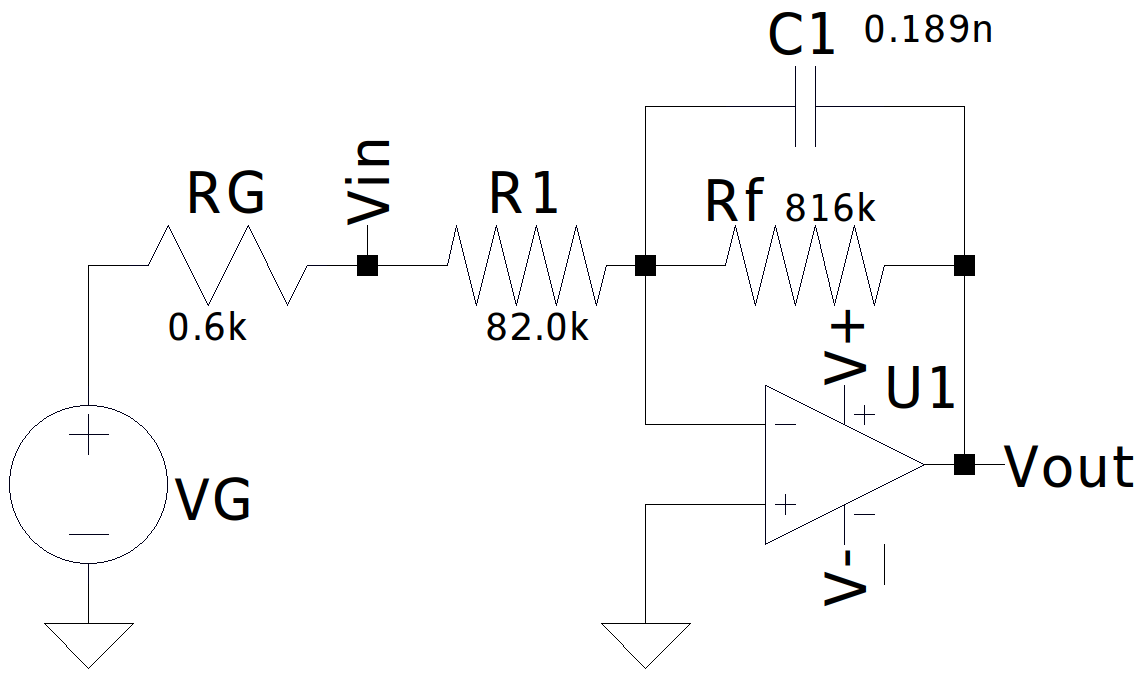
\includegraphics[width=0.38\textwidth]{../preamp/images/circuito}
  %\\caption{\footnotesize Schema a variabili concentrate del circuito preamplificatore.}
  %\\vspace{-10pt}
%\end{wrapfigure}\label{fig:preamp_circuito}%-----------------------------
funzioni incluso nel Picoscope in modo da
generare un impulso di tensione negativo di $-1\V$, partendo da un'quadra e
configurando il duty cycle al $99.5 \%$. In questo modo, selezionando una
frequenza di $1\kHz$, si ottiene una durata dell'impulso di $5\,\si{u\s}$ e,
tenendo conto della resistenza $R_{\text{in}}$ in serie, si può interpretare
come un impulso di corrente con una resistenza in parallelo, simulando quindi
l'output di un rilevatore di radiazione. Si nota però che, a causa dei limiti
tecnici del PicoScope 2204A, la durata del segnale non è stabile e non si presenta
come un'onda quadra perfetta, ma appare smussata.
Tutte le misure vengono quindi eseguite mettendo prima in pausa l'acquisizione
del segnale e si assume come valore del priodo quello nominale, con un'incertezza
sistematica  $\sigma_{T}=3\%$.%------------------------------
\renewcommand{\arraystretch}{1.1}
\begin{table}
\centering
\setlength{\tabcolsep}{10pt}
\begin{tabular}{ |c|c|c|  }
\hline
\multicolumn{3}{|c|}{Misure dirette dei componenti del circuito} \\
\hline
Label      & Valore & F.S.\\
\hline
$R_{1}$ & $82.0 \pm 0.4\,\si{k\Omega}$ &$200\,\si{k\Omega}$ \\
$R_{\text{f}}$ & $816 \pm 4\,\si{k\Omega}$ &$2\,\si{M\Omega}$ \\
$C_{\text{f}}$ & $0.189 \pm 0.004\,\si{n\farad}$ &$2\,\si{n\farad}$ \\
\hline
\end{tabular}
\caption{\footnotesize Si mostrano in tabella i valori e le incertezze delle componenti usate
  in questa sezione, misurati con il multimetro Tenma. È stato riportato anche il fondo scala
  usato.}\label{tab:preamp_misure}
\end{table}
%-------------------------------------
\noindent Infine, si configura l'oscilloscopio
in modalità $DC$, in quanto i circuti utilizzati possono generare una tensione
continua sotto i segnali che si vuole analizzare. Si decide inoltre di
considerare come zero delle misure di tensione proprio questa baseline,
utilizzando due cursori per ogni misura e registrando la differenza tra di essi.
\\

\begin{wrapfigure}{r}{0.4\textwidth}
  \centering
  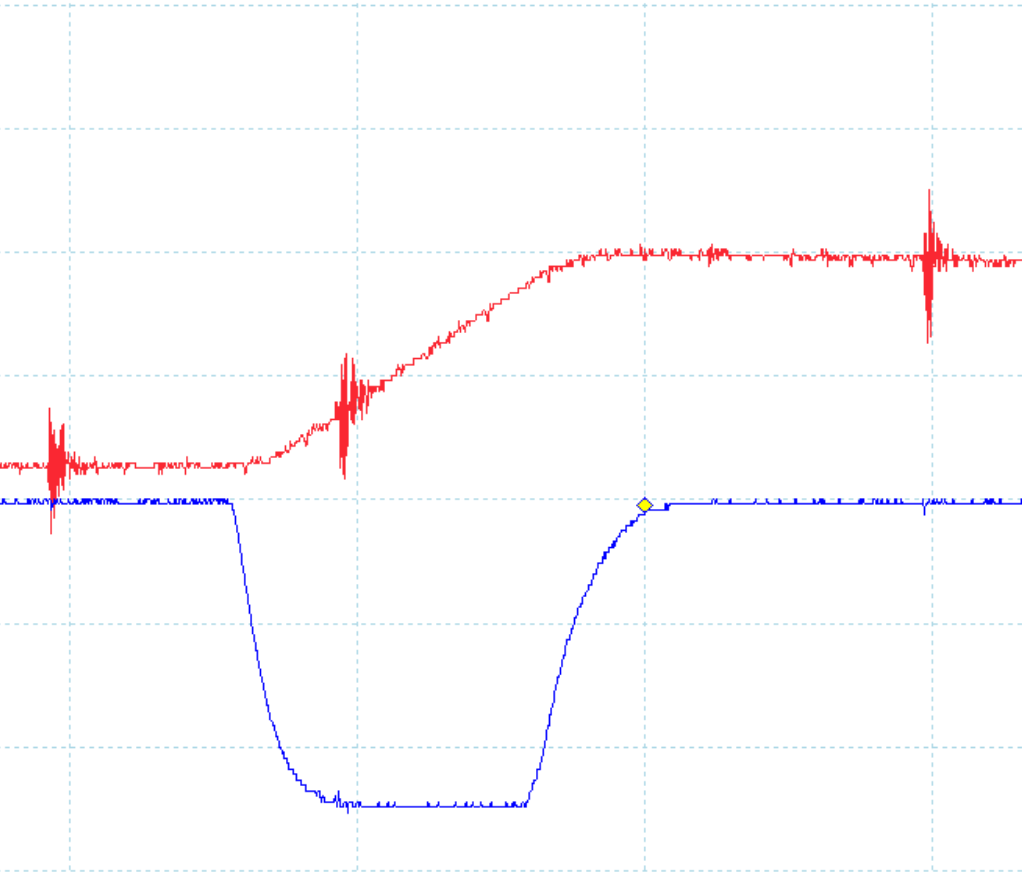
\includegraphics[width=0.38\textwidth]{../preamp/images/screen_interferenza1}
  \caption{\footnotesize Screenshot che mostra il primo fenomeno di interferenza ($0.4\V/div$ e $5\,\si{u\s}/div$).}\label{fig:preamp_interferenza1}%-----------------------------
  \vspace{-35pt} % This removes the white box on the second page
\end{wrapfigure}
\noindent Si vuole infine riportare la presenza di fenomeni di interferenza che sono stati osservati a intervalli irregolari nel corso dell'esperienza: il primo, come mostrato
in Figura~\ref{fig:preamp_interferenza1}, si presenta come una serie di pacchetti d'onda ad alta frequenza
e distanziati $5-10 \,\si{u\s}$, che non ha influenzato particolarmente l'acquisizione
delle misure; la seconda tipologia di interferenza, più rara, verrà invece mostrata in Figura~\ref{fig:shaper_undershoot}, e come si spiegherà nella Sezione~\ref{sec:shaper_pz}, ha disturbato il
segnale al punto da complicare sensibilmente la presa dei dati. Dopo aver controllato con attenzione che tutti i cavi facessero bene contatto, si è giunti alla conclusione che l'origine delle interferenze sia da attribuire ai numerosi dispositivi elettronici presenti
in prossimità del circuito.

\subsection{Analisi del ciruito}\label{sec:preamp_analisi}
Il sistema costituito dal generatore reale (di resistenza
$R_{G}\approx 0.6\kOhm$) e dalle capacità parassite dei cavi in ingresso
($C_{i}\approx 100\,\si{p\farad} $)  presenta una frequenza di taglio di circa
$3 \,\si{M\Hz}$, molto più grande delle frequenze in gioco e pertanto il
generatore può essere assunto ideale.
Risolvendo il circuito del preamplificatore (assumendo ideale l'amplificatore
operazionale) si ottiene la funzione di
trasferimento
\begin{align}\label{eq:preamp_tau}
  \text{A}(s) &= - \frac{1}{R_{1}\,C_{\text{f}}} \, \frac{1}{s+1/\tau_{\text{pre}}}
  &
    \tau_{\text{pre}} &=R_{\text f}\, C_{\text f}=0.154 \pm 0.004\,\si{\milli\second}
\end{align}
da cui si prevede che il circuito si comporterà come un filtro passa basso con
frequenza di taglio
\begin{align}\label{eq:preamp_ft}
  f_{t}&=\frac{1}{2\pi\,\tau_{\text{pre}}}=1.03\pm 0.02\,\si{k\Hz}
  &
    \sigma_{f_{t}}=f_{t}\, \sqrt{
    {\left(\frac{\sigma_{R_{f}}}{R_{f}}\right)}^{2}+
    {\left(\frac{\sigma_{C_{f}}}{C_{f}}\right)}^{2}}
\end{align}
Si prevede inoltre che la risposta del circuito ad un segnale a gradino
sia, per tempi inferiori al periodo $T$, una crescita lineare proporzionale
alla carica $Q_{\text{in}}(t)$ che raggiunge il preamplificatore
\begin{align}\label{eq:preamp_vout}
  V_{\text{out}}& = - \frac{Q_{\inp}(t)}{C_{\text f}} = - \frac{I_{\text{in}}\,}
                  {C_{\text f}}\,t = -\frac{V_{\inp}}{R_{1}}\frac{t}{C_{\text f}}
  &
  \text{per }& 0 < t < T
\end{align}
dove $I_{\text{in}}$ rappresenta la corrente che scorre nella resistenza di
ingresso $R_{1}$.
Per tempi maggiori invece, ci si aspetta una decrescita esponenziale
\begin{align}\label{eq:preamp_vout_exp}
  V_{\text{out}}& = - \frac{Q_{C}}{C_{\text{f}}}\,e^{-\frac{t}{\tau_{\text{pre}}}}=
                  - \frac{I_{\text{in}}\,T}{C_{\text{f}}}\,e^{-\frac{t}{\tau_{\text{pre}}}}
  &
   \text{per }& t> T
\end{align}
dove $Q_{C}$ rappresenta la carica totale accumulata dal preamplificatore.
Si prevede quindi di osservare una tensione massima $V_{\text{max}}=Q_{C}/C_{\text f}$ e, per verificare il funzionamento dell'apparato sperimentale, si confronta
questo valore con una misura diretta della tensione massima rilevata
dall''oscilloscopio: si manda in ingresso un segnale a gradino di periodo
$T=5\,\si{u\s}$ con ampiezza $-1\V$ e si utilizzando i cursori veritcali per
misurare il massimo del segnale in $V_{\text{out}}$ rispetto alla baseline.
Si associa quindi al valore letto l'incertezza sistematica sommata
quadraticamente all'errore di lettura. Sebbene tecnicamente le misure di tensione
siano riferite a due cursori, si sceglie di non considerare il termine $\sqrt 2$ nella
propagazione per evitare sovrastime eccessive dell'errore, in quanto l'oscilloscopio misura
la differenza tra due cursori con una precisione paragonabile a quella della singola misura
\begin{align}\label{eq:v_osc_err}
  V_{\text{max}}^{sp}&=0.344 \pm 0.006 \V
  &
  \sigma_{V_{\text{max}}^{sp}}&=\sqrt{ {\left(\sigma_{L}\times \text{scala}\right)}^{2}+
  {\left(\sigma_{K}\times V_{\text{max}}^{sp}\right)}^{2}}
\end{align}
dove $\sigma_{K}=1.7\%$ rappresenta l'errore di scala fornito dal costruttore (assumendo una distribuzione uniforme) mentre $\sigma_{L}$ rappresenta l'errore di lettura che si attribuisce principalmente alla discretizzazione del segnale e si calcola quindi a partire dalla risoluzione
dell'oscilloscopio $\Delta_{L}= 1/2^{n}$. Nel caso del Picoscope 2204A, vale $n=8\,\text{bits}$ e si ottine equindi $\sigma_{L}=0.002$.
Dalle considerazioni precedenti, invece, segue che la tensione massima attesa vale
\begin{align}
  V_{\text{max}}^{th}&=0.323 \pm 0.012 \V
  &
  \sigma_{V_{\text{max}}^{th}}&=V_{\text{max}}^{th}\,\sqrt{ {\left(\frac{\sigma_{R_{1}}}
                {R_{1}}\right)}^{2}+
 {\left(\frac{\sigma_{C_{\text{f}}}}
                {C_{\text f}}\right)}^{2}+
  {\left(\sigma_{T}\right)}^{2}}
\end{align}
dove, per semplicità, si è trascurato l'errore su $V_{\inp}$ e si assume il valore nominale del generatore. La compatibilità tra le due stime è $\lambda=1.5$, cioè discreta.

\subsection{Verifica della linearità del preamplificatore}\label{sec:preamp_lin}
Si vuole ora verificare la linarità della tensione massima di uscita $V_{\text{out}}$ del preamplificatore
rispetto alla carica in ingresso $Q_{\text{in}}$ (Equazione~\ref{eq:preamp_vout}).
Si modifica quindi la durata dell'impulso del generatore tra $5\,\si{u\s}$ e
$15\,\si{u\s}$ in modo da variare la
quantità di carica iniettata e si misura il massimo del segnale rilevato, sempre
rispetto alla baseline.

\subsubsection{Analisi Dati}\label{sec:pream_lin_an}
Per verificare la linearità del preamplificatore si vuole rappresentare i dati
acquisiti in un grafico ed effettuare un fit, per poi stabilire in base
all'andamento dei residui la validità dell'ipotesi. Alle tensioni (in ordinata)
si associa un errore calcolato come nell'Equazione~\ref{eq:v_osc_err}, considerando quindi
sia la componente sistematica che quella casuale dell'errore, in quanto le misure
sono state acquisite a scale diverse. Questo tuttavia introduce una correlazione
tra i dati di cui il fit non tiene conto e che porta ad una sottostima degli
errori dei parametri. Per quanto riguarda gli errori da associare alla carica
in ingresso $Q_{\text{in},i}=-\frac{V_{\text{in}}}{R_{1} }\,T_{i}$ (in ascissa) la situazione è più complicata. Essi infatti dipendono da
tre fattori: l'errore sulla resistenza $\sigma_{R_{1}}$, sulla tensione
$\sigma_{V_{\text{in}}}$ e sul periodo $\sigma_{T_{i}}$ del segnale in ingresso.
Tuttavia i primi due termini sono costanti per tutte le misure e l'errore
sul periodo è solo sistematico e quindi anch'esso porta un contributo costante.
Segue quindi che gli errori sulla carica sono totalmente correlati e non possono
quindi essere presi in considerazione durante il fit. Si decide allora di
calcolare due interpolazioni: in un primo momento si esegue la regressione lineare
della tensione in uscita $V_{\out}^{\text{max}}$ rispetto al periodo $T$, si ricava il coefficiente
angolare $b$ e si proietta l'errore di scala del periodo
secondo la formula
$\widetilde{\sigma_{b}}=\sqrt{ \sigma_{b,fit}^{2}+b^{2}\, \sigma_{T}^{2}}$. Si esegue
poi il fit di $V_{\text{out}}$ rispetto a $Q_{\text{in}}$, trascurando gli errori
delle ascisse per le considerazioni precedenti. Dal grafico dei residui, che non
dipende dagli errori sistematici, si valuta la linearità del preamplificatore, mentre, per dare una stima all'errore del coefficiente angolare $m$, si sfrutta la
sua relazione con la pendenza $b$ del primo fit
\begin{align}
  m&=\frac{b}{I_{\text{in}}}=\frac{R_{1}}{V_{\text{in}}}\, b
  &
    \sigma_{m} = m\,\sqrt{ {\left(\frac{\widetilde{\sigma_{b}}}{b}\right)}^{2}+
    {\left( \frac{\sigma_{R_{1}}}{R1}\right)}^{2} +
    {\left( \frac{\sigma_{V_{\text{in}}}}{V_{\text{in}}} \right)}^{2}}
\end{align}\label{eq:preamp_lin_eq}%--------------------------------------
In Figura~\ref{fig:preamp_fit_lin} vengono riportati i risultati del secondo fit, il cui grafico
dei residui evidenzia un'ottima distribuzione attorno allo zero e in generale una
buona stima degli errori sulle tensioni, indicata anche dall'errore a posteriori. Anche il chi quadro risulta in ottimo
accordo con l'aspettativa teorica ($\lambda=0.4$). Si conferma quindi l'ipotesi
di linearità della tensione massmia di uscita $V_{\text{out}}^{\text{max}}$ rispetto alla carica
$Q_{\text{in}}$ che raggiunge il preamplificatore.

\noindent Dalla prima interpolazione invece, dopo aver proiettato il contributo di scala
delle ascisse, si ottiene il coefficiente angolare $b=0.057\pm 0.002\V$ e, utilizzando
l'Equazione~\ref{eq:preamp_lin_eq}, si calcola il nuovo errore della pendenza
$m=4.7\pm0.2 \V$. Per l'Equazione~\ref{eq:preamp_vout}, l'inverso di questo coefficiente
angolare corrisponde alla capacità $C_{\text f}$ e infatti la stima $C_{\text{fit}}=0.215\pm0.009 \,\si{n\farad}$ è compatibile con il valore della capacità di feedback ottenuto da una misura diretta col multimetro, anche se
debolmente ($\lambda=2.5$). Tuttavia, l'Equazione~\ref{eq:preamp_vout} prevede anche che
l'intercetta del fit in Figura~\ref{fig:preamp_fit_lin} sia compatibile con lo zero, mentre
risulta $\lambda=5.9$. Si attribuisce questa anomalia alla presenza di errori
sistematici, visto l'ottimo andamento dei residui attorno allo zero (ricordando che essi non
sono affetti da erorri sistematici costanti). Avendo
però acquisito le misure di tensione rispetto alla baseline del segnale di fondo, si esclude la presenza di un errore di offset verticale delle ordinate. Inoltre,
avendo considerato le incertezze di scala delle tensioni nel fit e osservando che
errori di guadagno (costanti) delle ascisse non hanno effetto sull'intercetta,
si attribuisce lo sfasamento dell'intercetta ad un errore di
offset dei periodi. La scelta di attribuire solo un'incertezza sistematica ($\sigma_{T}=3\%$ del valore
nominale), spiegata nella Sezione~\ref{sec:preamp_config_sperim}, va infatti interpretata come un'assunzione
per semplificare i conti, più che un'analisi esaustiva dell'errore.
Si ricorda, infine, che avendo considerato gli errori sistematici
delle tensioni nei fit, si è introdotta una correlazione che porta ad una
sottostima degli errori e quindi a compatibilità peggiori. Si decide allora
di confermare l'ipotesi di linearità del preamplificatore, ma si ritiene
l'analisi svolta insufficiente per confermare la validità dell'Equazione~\ref{eq:preamp_vout}.
%------------------------------------
\begin{figure}[h]
\centering
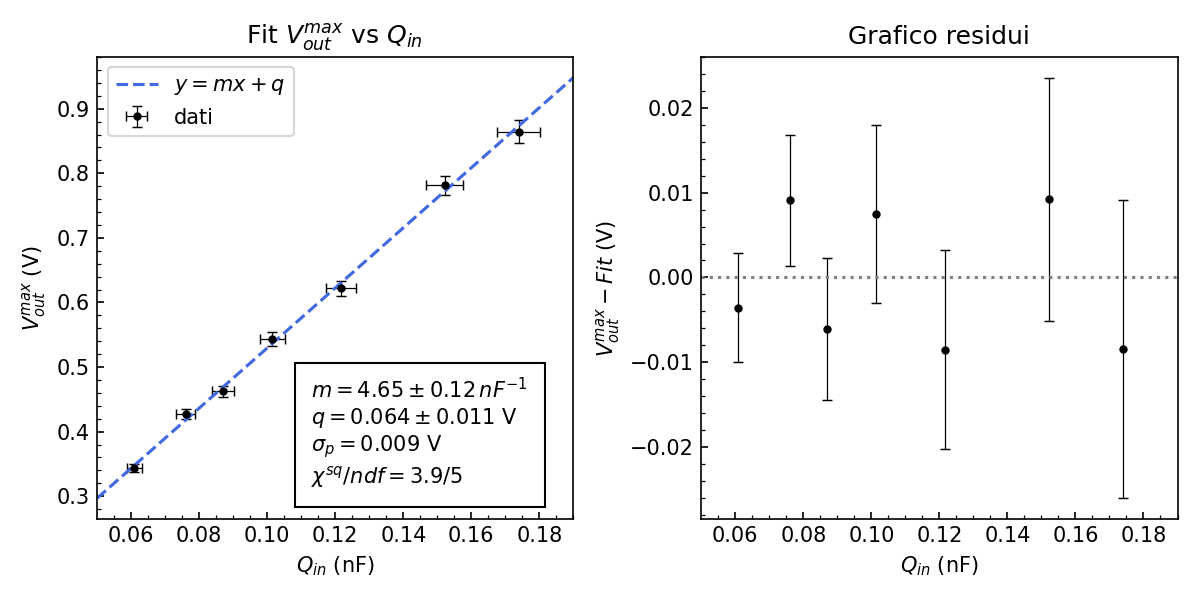
\includegraphics[width=0.8\textwidth]{../preamp/images/fit_lin}
\caption{\footnotesize A sinistra si mostrano i dati sperimentali e il fit della tensione massima in uscita rispetto alla carica in ingresso. Gli errori delle ascisse vengono riportati
  a scopo dimostrativo ma non vengono considerati nel fit, come spiegato. Le incertezze sui parametri
  mostrate sono quelle ottenute dall'interpolazione. Inoltre, a destra, viene riportato il grafico dei residui.}\label{fig:preamp_fit_lin}
\end{figure}
%------------------------------------

\subsection{Tempo Caratteristico del Preamplificatore}\label{sec:preamp_ft}
In questa sezione ci si concentra sulla fase di scarica del segnale. Con l'obiettivo di stimare
il tempo caratteristico del preamplificatore a partire da un fit esponenziale (Equazione~\ref{eq:preamp_vout_exp}) e
da uno lineare, si manda in ingresso un onda quadra di periodo\footnote{Si segnala una svista in fase di acquisizione dati per cui il periodo dell'onda quadrata è stato impostato a $50\us$, diversamente da quanto detto.}  $T=5\,\si{u\s}$ e ampiezza $1\V$, e si misura la tensione in uscita $V_{\text{out}}$ in corrispondenza di istanti di tempo $t$ diversi.

\subsubsection{Analisi Dati}\label{sec:preamp_ft_analisi}
Alle misure di tensione viene associato l'erore di lettura dell'oscilloscopio,
analogamente a quanto svolto nella sezione precedente. All'istante di tempo
$t$ si associa invece un errore (massimo) di lettura pari a $1/10$ dei $secondi/divisione$ corrisponendi alla scala selezionata. Per evitare di
sovrastimare l'errore si assume ora una distribuzione triangolare, ottenendo quindi un errore di lettura di $\sigma_{L}=0.04\,\text{div}$. L'errore di guadagno sui
tempi fornito dal costruttore è dello $0.01\%$ e si assume quindi trascurabile.
Gli errori relativi dei tempi così calcolati sono generalmente di un ordine di grandezza inferiore rispetto alle incertezze relative delle tensioni. Si decide quindi
di effettuare il fit esponenziale $y=a+b \exp(t\,c)$ considerando solo gli errori delle ordinate. I risultati dell'interpolazione e una simulazione
LTspice del circuito sono riportati in
Figura~\ref{fig:preamp_fit_exp_lin}: dal grafico dei residui si evidenzia un ottimo andamento
attorno allo zero ma una leggera sovrastima degli errori, indicata anche
dalla deviazione standard a posteriori e dal chi quadro eccessivamente basso.
L'inverso del parametro $c$ rappresenta la prima stima sperimentale del
tempo caratteristico $\tau_{\text f,\text{exp}}= 0.16\pm 0.01\,\si{m\s}$, in ottima compatibilità con l'aspettativa teorica calcolata nell'Equazione~\ref{eq:preamp_tau} ($\lambda=0.2$).
Anche il parametro $a$ risulta perfettamente compatibile con lo zero
($\lambda=0.6$). Ci si aspetta infine che il parametro $b$ corrisponda
alla carica totale scalata dall'inverso della capacità di feedback
\begin{align}
  b_{th}=-\frac{Q_{C}}{C_{\text f}}& =-\frac{V_{\text{in}}\,T}{R_{1}\, C_{\text{f}}}=3.21 \pm 0.10 \V
  &
    \sigma_{b_{th}}& = b_{th}\,
                     \sqrt{{\left(\frac{\sigma_{V_{\text{in}}}}{V_{\text{in}}}\right)}^{2}+
                     {\left(\frac{\sigma_{R_{1}}}{R_{1}}\right)}^{2}+ {\left(\frac{\sigma_{C_{\text f}}}{C_{\text f}}\right)}^{2}+
                     \sigma_{T}^{2}}
\end{align}
dove $V_{\text{in}}= 0.99\pm 0.02 \V$ viene misurato direttamente con l'oscilloscopio. Confrontando $b_{th}$ col valore
%------------------------------------
\begin{figure}[h]
\centering
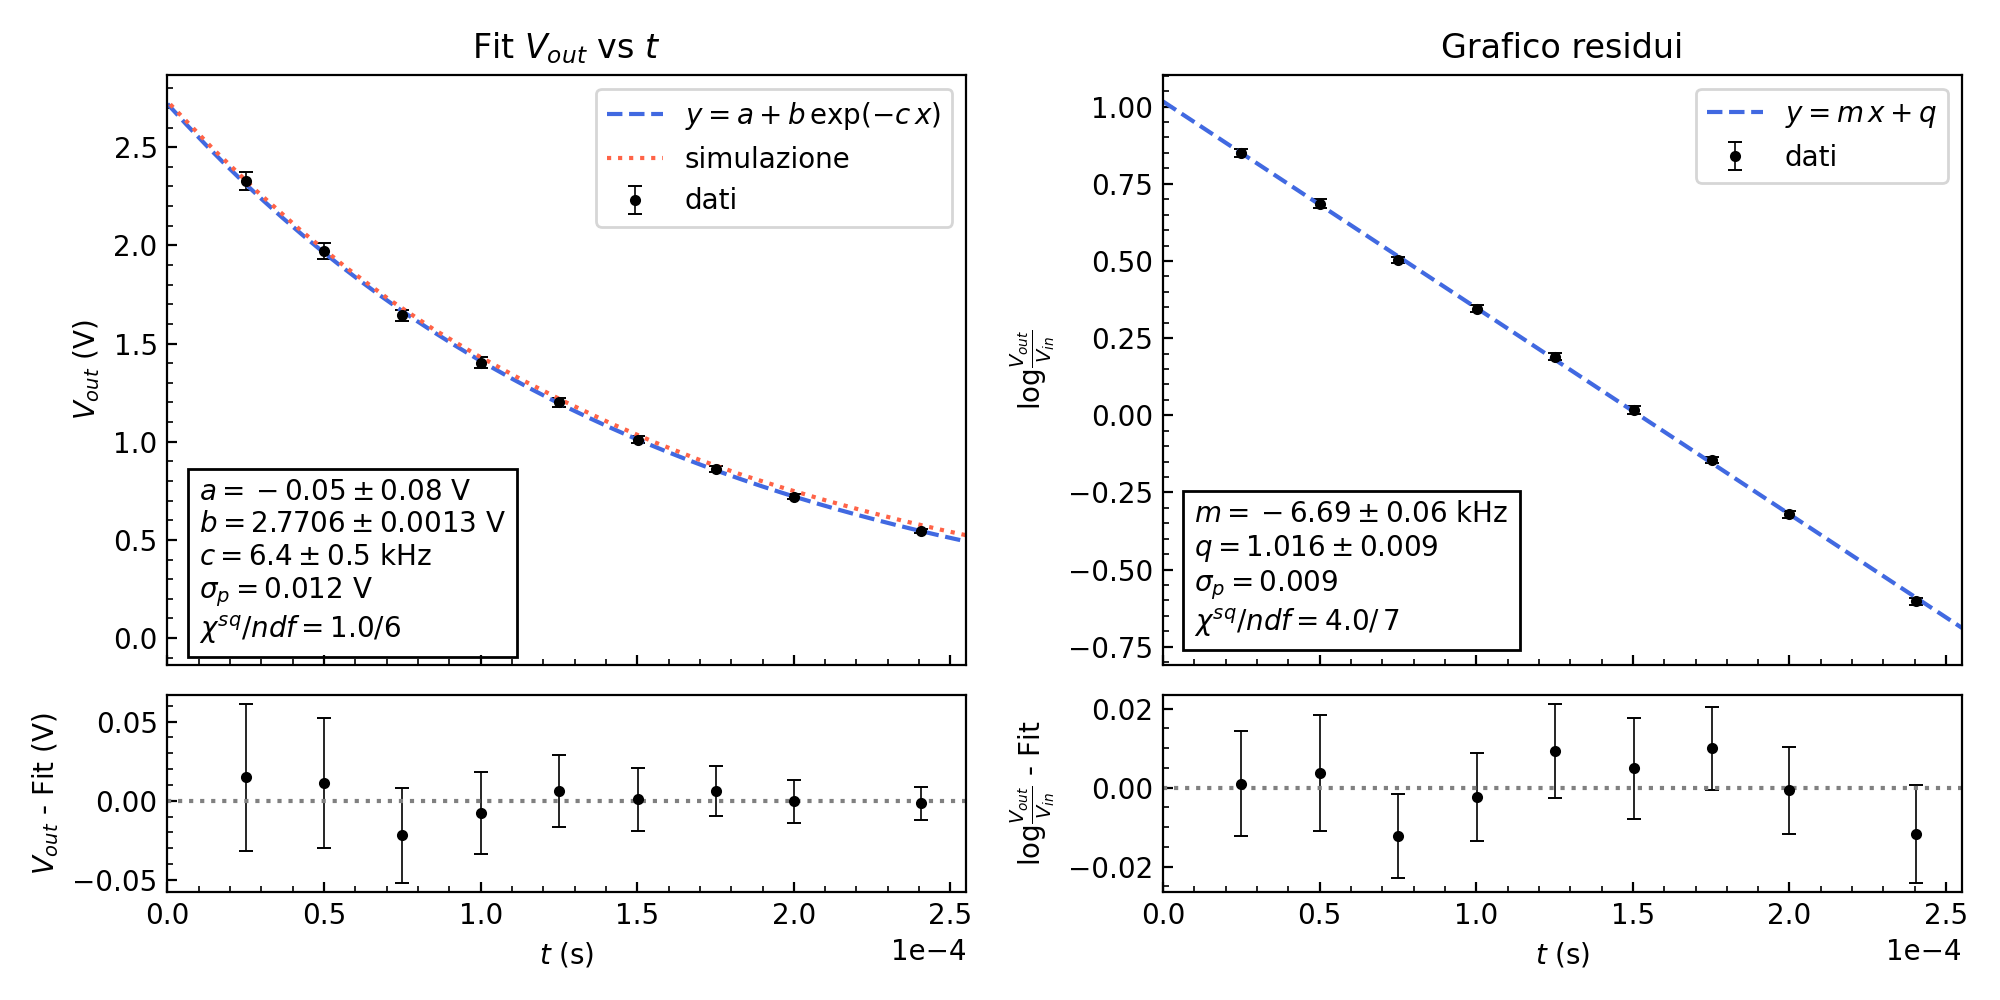
\includegraphics[width=0.9\textwidth]{../preamp/images/fit_exp_lin}
\caption{\footnotesize A sinistra si mostrano il fit esponenziale e la
  simulazione ottenuta con LTspice mentre a destra viene riportata l'interpolazione lineare. Sotto entrambi i grafici vengono mostrati anche gli andamenti dei residui.}\label{fig:preamp_fit_exp_lin}
\end{figure}
%------------------------------------
\noindent ottenuto dal fit si
riscontra che tali valori sono incompatibili ($\lambda=4.4$). Visto il buon
accordo dei dati con la simulazione LTspice, si attribuisce questa
discrepanza alla correlazione introdotta considerando gli errori sistematici
sulle tensioni, che porta ad una sottostima dell'errore dei parametri.
\noindent Si vuole ora ottenere una nuova stima del tempo caratteristico a partire da
un fit lineare, considerato più robusto rispetto all'interpolazione
non lineare. Dopo aver diviso entrambi i membri per $V_{\text{in}}$ in modo da rendere
adimensionale l'argomento del logaritmo, si linearizza l'Equazione~\ref{eq:preamp_vout_exp}
ottenendo la relazione
\begin{align}
  y & = \log{\left|\frac{V_{\text{out}}}{V_{\text{in}}}\right|} = -\frac{t}{\tau}+\log{\left(\frac{T}{R_{1}C_{\text f}}\right)}
  &
    \sigma_{y}&= |y| \sqrt{{\left(\frac{\sigma_{L}\times \text{scala}_{in}}{V_{\text{in}}}\right)}^{2}+
    {\left(\frac{\sigma_{L}\times \text{scala}_{out}}{V_{\text{out}}}\right)}^{2}}
\end{align}
dove nel calcolo dell'errore sulle y si sono trascurati i contributi dell'errore di scala
di $V_{\text{in}}$ e $V_{\text{out}}$ in quanto, per le proprietà del logaritmo, si trasferiscono sull'intercetta.
I risultati del fit lineare sono riportati in Figura~\ref{fig:preamp_fit_exp_lin}, da cui si
osserva una buona distribuzione dei residui attorno allo zero e una
discreta stima dell'errore. Dall'inverso del coefficente angolare si ricava
la seconda stima sperimentale del tempo caratteristico $\tau_{\text{lin}}=0.1496\pm0.0013 \,\si{m\s}$. Tale valore risulta compatibile con la stima
ottenuta dal fit esponenziale ($\lambda=1.0$) ed è in ottimo accordo anche con il valore
ricavato dall'Equazione~\ref{eq:preamp_tau} ($\lambda=1.0$). Si preferisce la stima
ottenuta dal fit lineare in quanto meno affetta da errori sistematici.

\subsection{Risposta in frequenza del Preamplificatore}\label{sec:preamp_bode}
In questa sezione si approfondisce la risposta in frequenza del preamplificatore, registrando il massimo della tensione in uscita
$V_{\text{out}}$ per segnali sinusoidali di ampiezza $1\V$
e di frequenze comprese tra $10\,\si{\Hz}$ e $100\,\si{k\Hz}$. Dal grafico di Bode si ottiene poi una stima della
frequenza di taglio del circuito.

\subsubsection{Analisi Dati}\label{sec:bode_analisi}
Per realizzare il grafico di Bode (Figura~\ref{fig:preamp_fit_bode}) si esprime la funzione di trasferimento
in decibel
\begin{align}
  H(dB) &= 20\log_{10}{\left(\frac{V_{\text{out}}}{V_{\text{in}}}\right)}
  &
    \sigma_{H}(dB) = 20\,\log_{10}{(e)}\,\sqrt{{\left(\frac{\sigma_{L}\times \text{scala}_{in}}{V_{\text{in}}}\right)}^{2}+
    {\left(\frac{\sigma_{L}\times \text{scala}_{out}}{V_{\text{out}}}\right)}^{2}}
\end{align}
%------------------------------------
\begin{figure}[h]
\centering
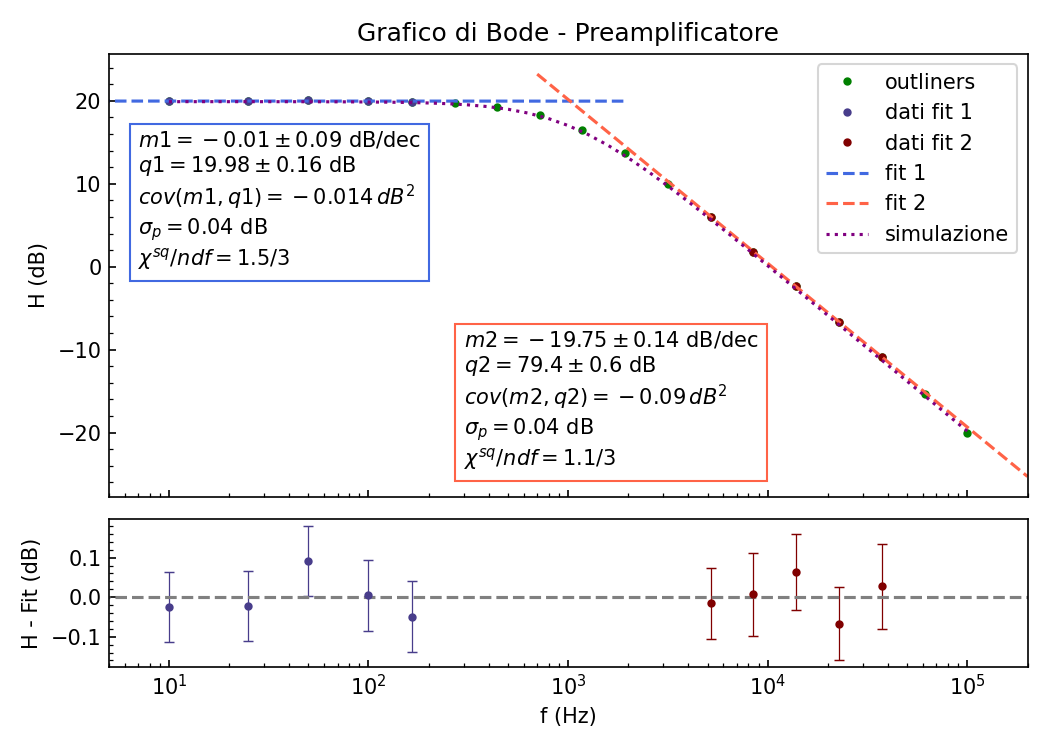
\includegraphics[width=0.7\textwidth]{../preamp/images/fit_bode}
\caption{\footnotesize Grafico di Bode del preamplificatore. Oltre ai dati sperimentali, si mostrano le due interpolazioni coi relativi
grafici dei residui e outliners (in verde). Vengono presentati anche i risultati di una simulazione (in viola).}\label{fig:preamp_fit_bode}
\end{figure}
%------------------------------------
Le frequenze vengono mostrate in scala logaritmica e si assume che la
loro incertezza sia trascurabile.
 Nella Figura~\ref{fig:preamp_fit_bode} si mostrano anche i
risultati di una simulazione del circuito che evidenzia un buon accordo per tutte le frequenze sia con i dati sperimentali che con le previsione teoriche: come spiegato in Sezione~\ref{sec:preamp_analisi} il circuito si comporta come un filtro passo basso e infatti per frequenze inferiori a $\approx 1\kHz$ la funzione di trasferimento
è approssimabile ad una retta di pendenza compatibile con lo zero (rappresentata in blu in Figura~\ref{fig:preamp_fit_bode}). A frequenze più alte invece,
la funzione di trasferimento decresce come una retta con pendenza
di circa $20 \,dB$ (in rosso).
\noindent L'intersezione tra le due rette fornisce una stima
della frequenza di taglio del circuito
\begin{align}
  f_{t}&=\frac{q_{1}-q_{2}}{m_{2}-m_{1}}=1.02\pm 0.03\,\si{k\Hz},
  &
    \sigma_{f_{t}}&= f_{t}\,\sqrt{  \frac{\sigma_{q_{1}}^{2}+\sigma_{q_{2}}^{2}}{{(q_{1}-q_{2})}^{2} } +
                    \frac{\sigma_{m_{1}}^{2}+\sigma_{m_{2}}^{2}}{{(m_{2}-m_{1})}^{2} } +
                    2\frac{\text{cov}(q_{1},m_{1})+\text{cov}(q_{2},m_{2})}{(q_{1}-q_{2})(m_{2}-m_{1})} }
\end{align}
compatibile sia con l'aspettativa teorica calcolata in Equazione~\ref{eq:preamp_ft} ($\lambda=0.2$) che con la frequenza ottenibile dalla stima del tempo caratteristico
della sezione precedente $f_{t,\text{lin}}= 1.064\pm 0.010\kHz$ (in questo caso vale $\lambda=1.5$).
